\section{Concept of LEM Simulation Platform}
\label{sec:concept_of_lem}
To start off, this section brings together the previous sections \ref{sec:about_blockchain} and \ref{sec:btm},
and explains how the BTM and a blockchain interact to implement the BLEMS.
Finally, this section gives an example of a LP in terms of energy efficient demand side management of households. 

First, in the presented BTM in section \ref{sec:btm}, independent, self-interested agents trading bundled resources
in a double-auction market. 
In case of the BLEMS, the agents of the BTM represent households that 
trade independently and self-interested bundles of energy resources to minimize their monetary expense 
through optimally scheduling the operation and energy consumption 
of all energy consuming appliances.

Second, blockchain is introduced as the applied ICT of the BLEMS. 
As previously mentioned, the implementation of LEM needs local distributed control and 
management techniques, which can be addressed by the blockchain technology.
This implies that the respective households submit and receive all relevant data, information, and payments via a blockchain. 
Moreover, the double-auction market which enables households to trade their energy bundles is operated by a dealer.
In turn, the dealer is implemented by a smart contract in conjunction with a conventional software client. 
The dealer's smart contract contains all relevant information regarding the market mechanism, like submitted orders, trades, 
dealer's inventory, and market prices. 
Therefore, households exclusively communicate with the dealer's smart contract. 

\begin{figure}[htbp]
    \centering
    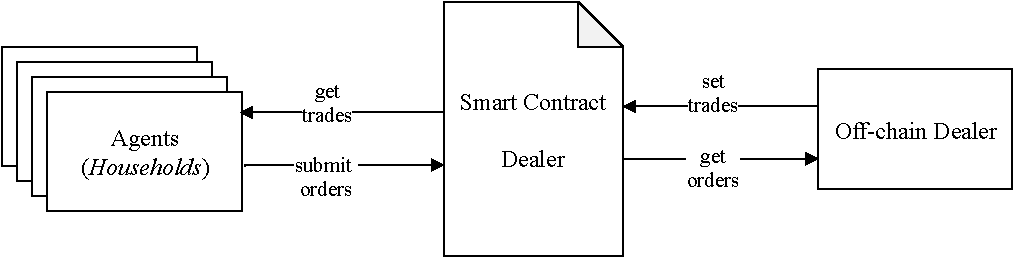
\includegraphics[width=.85\linewidth]{./figures/concept_lem.pdf}
    \caption{Presentation of the applied communication}
    \label{figure:concept_lem}
\end{figure}

As can be seen in Figure \ref{figure:concept_lem}, the households submit their orders to the dealer's smart contract. 
Afterwards, the dealer's conventional software client, labeled as \textit{off-chain} dealer in the Figure, fetches all existing orders contained in the smart contract
and solves the MMP.
Secondly, the off-chain dealer updates all relevant information in the smart contract, for instance 
the settled orders, the trades, the new market prices, and the resource inventory.
Finally, the households get their respective trades from the dealer's smart contract. 

Nevertheless, the off-chain dealer is necessary due to the complex and costly calculation of the MMP.
As mentioned in section \ref{sec:transaction}, each transaction consumes gas. Additionally, each mathematical operation in a smart contract
increases the amount of gas to be paid for the respective transaction. As a consequence, implementation and execution of the MMP
in the smart contract itself would be hard to realize and associated with high transaction costs. 

Hence, a well-designed smart contract should move computational complexity off-chain
and focus more on updating state in the contract \shortcite{calculate_cost_eth}. A balance between on-chain
and off-chain complexity should be found.

In addition, the BLEMS applied the synchronous call market, which means that the dealer executes the MMP exclusively after all agents 
have submitted their orders.
Likewise, we stated that smart contracts are only active and run if they called by a transaction,
wherefore they never run on his own or in the background.
For this reason, a mechanism is necessary which triggers the execution of the 
MMP, for wich the implementation of the off-chain dealer is also suitable.

So far, this section presented the basic idea and concept of the BLEMS
and explained the necessity of all existing components. In the following section \ref{sec:implementation}, 
the technical implementation is described in detail. 

However, we stated earlier in this section that the agents of the BTM represent households
that trade bundles of energy resources to minimize the monetary expense. 
In section \ref{sec:btm_problem_overview}, we introduced the individual LPs of the agents.
Further, we explained in section \ref{sec:agent_bidding} that a rational agent will choose an improving bundle for 
trading which leaves his wealth level on the same level or better off and defined the selection of such a bundle 
as the BDP.
Finally, to embed the BTM into the topic of LEM, we need to define 
a LP which depicts the energy efficient demand side management of households.

\subsection{Demand Side Management of a Household}
This subsection will embed the BTM into the topic of LEM. 
Therefore, we develop an exemplary LP in terms of energy efficient demand side management of households. 
The objective of the households is to minimize their monetary expense regarding energy consumption depending
on several constraints, which ensures the sufficient provision of energy at all times.

\shortciteA{Chen2013} developed such a LP for demand side management of households, on which the following
presented model is based. 

First, we introduce all relevant variables. Let $a$ denotes an appliance, and $A$ the set of all existing appliances in a household.
In that case, an appliance constitutes energy consuming items, e.g. washers, refrigerators, plug-in hybrid vehicles, etc.
Next, the variable $x_{a}$ denotes the energy consumed by an appliance $a$ to a given point in time. 
Further, each appliance $a \in A$ has a maximum energy level that is defined as rated power and described by $P_{a}$.
Additionally, it exists a limit on the total energy consumed by various appliances of a household. This total energy consumption limit is described by $L_{A}$. In case the total energy consumption limit is exceeded, the power network of the household will be tripped out.
Moreover, a household consumes, on the one hand, solar energy from
\textit{photovoltaic systems (PV)} and on the other hand energy from the electrical grid. 
If households do not consume solar energy directly, they have the opportunity to 
store it in batteries, or export it back to the main power grid if the battery is full.
Let $e_{g}$ denote the energy used from the electrical grid, and $e_{s}$ the energy produced by the PV.
In addition, let $p_{g}$ and $p_{s}$ denote the unit price of the energy from the electrical grid and solar energy.
Furthermore, we describe the solar energy used by all appliances of a household as $y_{s}$, the consumed battery energy 
as $y_{b}$ and the remaining solar energy which is not used by the household appliances and stored in the battery as $z_{b}$.

Finally, we developed the following LP for optimization of the household monetary expense.

\begin{equation}
 \begin{array}{ll@{}ll}
 \text{min} & \displaystyle p_{g} \cdot e_{g} + p_{s} \cdot e_{s} &\\
 \text{s.t.}& \displaystyle \sum\limits_{a \in A}^{} x_{a} \leq L_{A} \\
                    & \displaystyle x_{a} \leq P_{a}, \quad \forall a \in A \\
                    & \displaystyle \sum\limits_{a \in A}^{} x_{a} = y_{s} + y_{b} + e_{g} \\
                    & \displaystyle y_{s} + z_{b} \leq e_{s}
 \end{array}
\end{equation}

\clearpage
In the table below, all applied variables of the developed LP are listed:

\begin{longtable}{c|l}
	\caption{Applied variables in LP for optimization of the household monetary expense} 
	\label{table:applied_variables_lp} 
	\\
	\textbf{Variable} & \textbf{Description} \\
	\hline
    $a$ & energy consuming appliance of household \\
	$A$ & set of all existing energy consuming appliances of household \\
	$x_{a}$ & consumed energy of an appliance $a$ \\
	$P_{a}$ & maximum energy level (rated power) of an appliance $a$ \\
	$L_{A}$ & total energy consumption limit of a household \\
	$e_{g}$ & energy used from the electrical grid \\
	$e_{s}$ & energy produced by PV \\
	$p_{g}$ & unit price of energy from electrical grid \\
	$p_{s}$ & unit price of energy from PV \\
	$y_{s}$ & solar energy used by all appliances of a household \\
	$y_{b}$ & consumed batterie energy by all appliances of a household \\
	$z_{b}$ & remaining unused solar energy stored in the batterie \\
\end{longtable} 

As mentioned earlier,
the objective of the respective households is to minimize
their monetary expense regarding energy consumption.
The term $p_{g} \cdot e_{g}$ denotes the costs for energy from the electrical
grid, whereas the term $p_{s} \cdot e_{s}$ denotes the costs for energy from PV. 

Besides, the first constraint ensures that the total energy consumption of all energy consuming
appliances of a household does not exceed the limit of $L_{A}$. 

Next, the second constraint describes the requirement that the consumed energy
for all existing appliances $a$ in a household is less or equal 
to the respective rated power $P_{a}$.

Further, the third constraint makes sure that the energy consumed by all appliances
of a household is the sum of the energy from the electrical grid, the solar energy from the PV system and the battery energy. This implies if the amount of solar and battery energy is not sufficient to cover the energy consumption of all appliances, external energy from the electrical grid will be used. Therefore, it is ensured that sufficient energy is available at all times.

Finally, the fourth constraint describes that the solar energy produced by the PV system is greater or equal to the sum of the consumed and stored solar energy. 
At times when the battery is fully charged and the energy consumption of the 
appliances are covered by solar energy, it is possible to sell the surplus of 
wasted solar energy.
Referring to the BTM, the first two constraints of the proposed linear
programming model constitutes the independent resources that are managed locally.
The shared resources are represented by 
the energy resources $e_{g}$ and $e_{s}$.
Therefore the respective households trade the following limited bundles.

\[
w=
  \begin{pmatrix}
e_{g} \\
e_{s}
  \end{pmatrix}
\]

Consequently, the objective of the LP is written in matrix-vector notation.

\begin{equation*}
 \begin{array}{ll@{}ll}
        \text{min} & \displaystyle p^{T} \cdot w
 \end{array}
\end{equation*}

where $p^{T}$ denotes the transposed price vector.

\[
p^{T} =
  \begin{pmatrix}
p_{g} &
p_{s}
  \end{pmatrix}
\]



To sum up, this subsection presented a simplified LP for demand side management of a household
that can be integrated into the proposed BTM.

Furthermore, the developed model should only serve as an inspiration and example
and has no claim to completeness. 
It is intended to illustrate how the presented framework can be adapted to enable the trading of energy resources in LEM. 

\clearpage